%% LaTeX2e class for student theses
%% sections/evaluation.tex
%% 
%% Karlsruhe Institute of Technology
%% Institute for Program Structures and Data Organization
%% Chair for Software Design and Quality (SDQ)
%%
%% Dr.-Ing. Erik Burger
%% burger@kit.edu
%%
%% Version 1.3.3, 2018-04-17

\chapter{Evaluation}
\label{ch:Evaluation}
Das Hauptziel dieser Masterarbeit ist es, eine Modellierung einer MOM mit expliziten Warteschlangen zu ermöglichen und anschließend in Performance-Analysen zu untersuchen. Um dieses Ziel zu erreichen wurde in \autoref{ch:modellierung} eine Modellierungsmethode vorgestellt mit der eine MOM modelliert und kalibriert werden kann. Die in \autoref{ch:mom} ausgemessenen Ergebnisse wurden dabei zum Kalibrieren der Modelle verwendet. Im Folgenden, soll die bisherige Arbeit evaluiert werden und dabei gezeigt werden, dass die definierten Ziele erreicht werden konnten. 

Die Ziele und die Bewertung, ob diese erreicht werden konnten werden mithilfe der Goal-Question-Metric (GQM) untersucht.
Die GQM-Methode \cite{gqm} spezifiziert Ziele für das zu evaluierende Konzept. Daraufhin werden zu den Zielen Fragen spezifiziert, mit denen die Erfüllung des Ziels überprüft werden soll. Schließlich werden Metriken festgelegt, durch die die Fragen beantwortet werden sollen. Aus \autoref{tab:gqm} können die Ziele, Fragen und Metriken entnommen werden, mit denen diese Masterarbeit evaluiert werden soll.

Ein Ziel, das mithilfe dieser Masterarbeit erreicht werden soll, ist die Modellierung von MOMs in Palladio zu ermöglichen. Das zweite Ziel ist es, Vorhersagen mithilfe der Performance-Analyse zu ermöglichen und dadurch die Entscheidungsfindung, welche MOM verwendet werden soll, bereits zur Modellierungszeit und aus Architekturperspektive zu verbessern. Die dazu definierten Fragen prüfen ob mithilfe der Modellierung sowohl Punkt-Zu-Punkt, als auch Publish/Subscribe-Kommunikation vorhergesagt werden können. Dabei dient der Fehler zwischen Messung und Vorhersage als Metrik. In der Literatur ist ein Fehler zwschen 35\% und 40\% akzeptiert \cite{error}.

Im Folgenden wird in \autoref{sec:specjms} der SPECjms2007-Benchmark vorgestellt, mit dem die Evaluierung durchgeführt wird. Anschließend werden in \autoref{sec:specjmsmodell} die PCM-Modellierung des Benchmarks beschrieben. Im Anschluss wird in \autoref{sec:specjmsmodellvorhersage} die Vorhersagegenauigkeit der Modellierung untersucht. Schließlich werden in \autoref{sec:evaluationzusammenfassung} die Ergebnisse zusammengefasst und diskutiert. 
\begin{table}
  \begin{tabular}{|l|l|}
    \hline
    \multicolumn{2}{|l|}{Ziel 1} \\
    \hline
    Zweck & Ermögliche \\
    Qualitätskriterium & eine wartbare und wiederverwendbare Möglichkeit  \\ 
    Prozess & eine MOM zu modellieren \\
    Sicht & aus Architekturperspektive \\
   
    \hline \hline
    \multicolumn{2}{|l|}{Ziel 2} \\
    \hline
    Zweck & Verbessere \\
    Qualitätskriterium & die Abwägung und Entscheidungsfindung  \\ 
    Prozess & beim Einsatz einer MOM \\
    Sicht & aus Architekturperspektive \\
    \hline \hline
    Frage 1 & Lässt sich die Latenz einer Nachricht für Punkt-Zu-Punkt \\
    & Kommunikation vorhersagen? \\
    \hline
    Metrik & Fehler in \% zwischen Messung und Vorhersage? \\
    \hline \hline
    Frage 2 & Lässt sich die Latenz einer Nachricht für Publish/Subscribe-\\
    & Kommunikation vorhersagen? \\
    \hline
    Metrik & Fehler in \% zwischen Messung und Vorhersage? \\
    \hline
  \end{tabular}
	\caption{\label{tab:gqm} Ziele, Fragen und Metriken für die Evaluierung, nach der GQM-Methode}
\end{table}


%\section{Systemanforderungen}
%\label{sec:systemanforderungen}
%Für das Evaluierungssystem wurden im Folgenden Anforderungen festgelegt.
%\begin{itemize}
%\item Das jeweilige System soll \textbf{Skalierung} erlauben. Dabei soll es zum einen möglich sein die Anzahl von Kommunikationspartnern zu erhöhen (\textit{horizontal}) als auch die Menge an Nachrichten die verschickt werden (\textit{vertikal}).
%\item Weitere \textbf{Konfigurationen} wie Nachrichtengröße, reihenfolgentreue, Duplikate, etc. sollten möglich sein.
%\item System soll möglichst \textbf{reales System} darstellen.
%\item Mindestens ein \textbf{Nachrichtenmodell} sollte unterstützt werden.
%\item Es sollten \textbf{verschiedene Interaktionstypen} unterstützt werden, wie Many-To-Many, Many-To-One, etc.
%\item Damit der Fokus der Masterarbeit auf den MOMs und ihrer Modellierung liegt, sollte das System \textbf{bereits vorhanden} und implementiert und modelliert sein.
%\end{itemize}

\section{SPECjms2007}
\label{sec:specjms}
Das für die Evaluierung verwendete System ist das im SPECjms2007-Benchmark verwendete Testsystem \cite{Sachs2013}. Der Benchmark stellt eine reale Anwendung dar und umfasst eine Reihe verschiedener Interaktionen, die sowohl Punkt-zu-Punkt- als auch Publish/Subscribe-Nachrichten umfasst. Das Hauptziel des SPECjms2007-Benchmarks ist es, einen Standard-Workload bereitzustellen, der die Leistung und Skalierbarkeit von JMS-basierten nachrichtenbasierten Middleware-Plattformen bewertet. Bei dem System handelt es sich um ein Lieferkettenmanagement für eine Supermarktkette. Der Benchmark verwendet verschiedene Nachrichtentypen und verwendet Nachrichten verschiedenen Größe. Für die Masterarbeit liegt sowohl die Implementierung des Benchmarks, als auch eine Modellierung aus einer früheren Arbeit von Christoph Rathfelder \cite{Rathfelder2013} vor. Dieses System wird für die Evaluierung verwendet werden und wird im Folgenden beschrieben. 

\subsection{Anwendungsszenario}
Das gewählte Anwendungsszenario bildet die Lieferkette eines Supermarktunternehmens ab. In \autoref{img:specjmsInteraction} sind die beteiligten Rollen abgebildet und wie sie miteinander kommunizieren. Die beteiligten lassen sich wie folgt gruppieren: 
\begin{itemize}
    \item \textbf{Hauptquartier} (HQ): Für die Buchhaltung des Unternehmens verantwortlich. Beobachtet den Geld und Warenfluss im System. Verwaltet Informationen über Waren und definiert Preise.
    \item \textbf{Supermarkt} (SM): Verkauft Waren an Kunden. Im Benchmark liegt der Fokus auf der Verwaltung der eigenen Warenlager. Jeder SM ist mit einem Vertriebszentrum verbunden.
    \item \textbf{Vertriebszentrum} (DC): Beliefert SM mit Waren. Ein DC nimmt Aufträge von SMs an und liefert diese. Wenn ein DC die Waren nicht vorrätig hat, werden diese Waren von einem Zulieferer angefordert. Außerdem sind DCs dafür verantwortlich Verkaufsstatistiken an das HQ zu senden.
    \item \textbf{Zulieferer} (SP): SPs sind nicht Teil des Supermarktunternehmens. Jeder SP bietet eine bestimmte Art von Waren an. Diese werden an DCs geliefert, wenn angefordert.
\end{itemize}

\begin{figure}
\center
  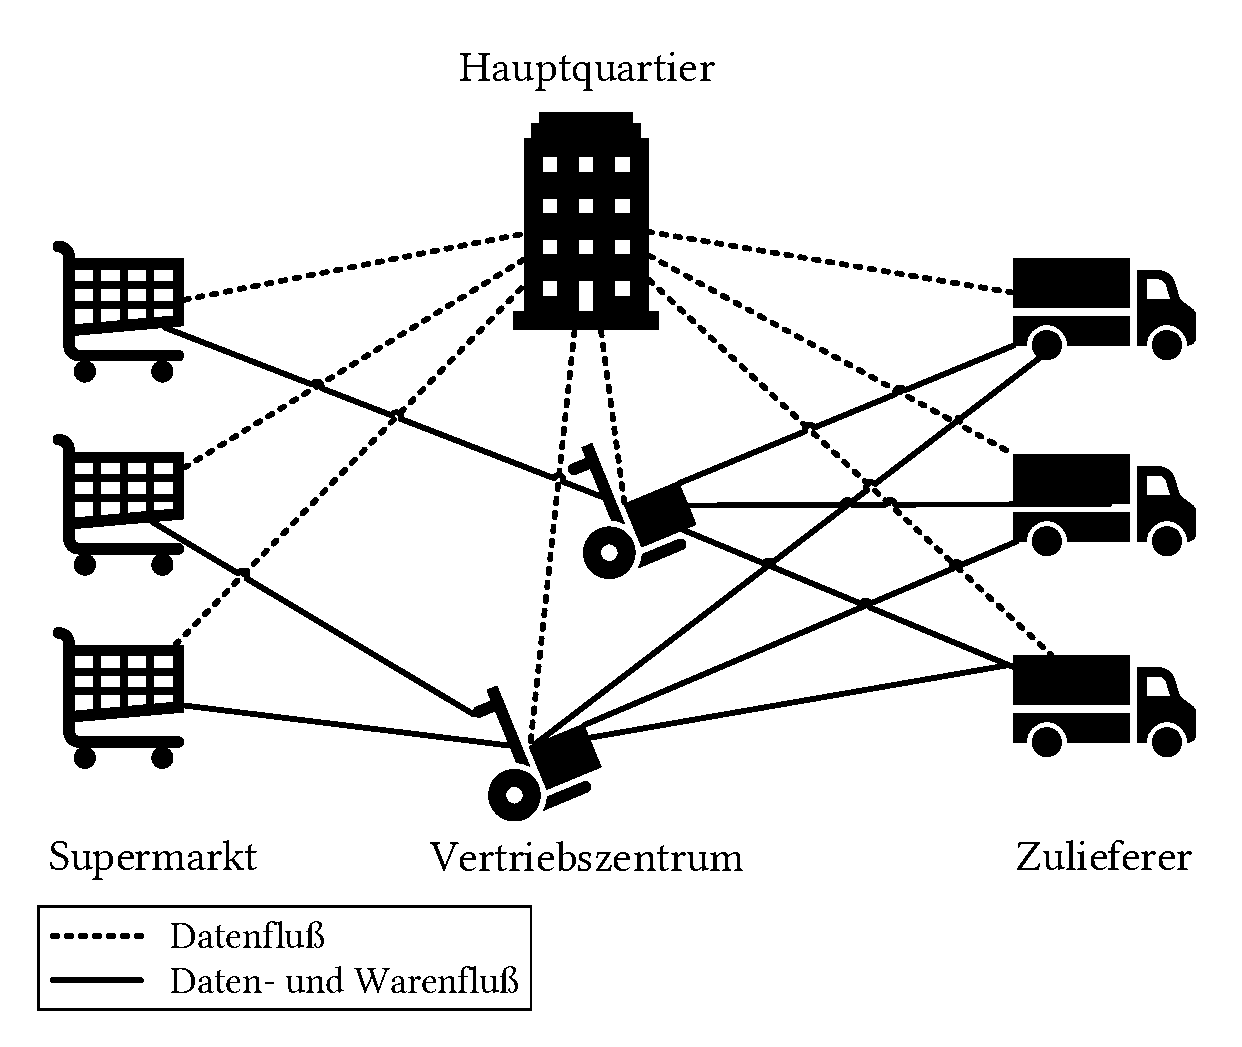
\includegraphics[width=0.7\textwidth]{images/evaluation/specjms/specjmsOverview.pdf}
  \caption{Anwendungszenario des SPECjms2007-Benchmark}
  \label{img:specjmsInteraction}
\end{figure}

\subsection{Interaktionen und Kommunikation}
Der SPECjms2007-Benchmark sieht insgesamt sieben verschiedenen Interaktionsmöglichkeiten vor: 
\begin{enumerate}
    \item Bestell- und Versandabwicklung zwischen SM und seinem DC (\emph{Punkt-Zu-Punkt}).
    \item Bestell- und Versandabwicklung zwischen DC und seinen SPs (\emph{Punkt-Zu-Punkt und Publisher/Subsciber}).
    \item Preisaktualisierung (\emph{Publisher/Subsciber}).
    \item Inventurmanagmenet (\emph{Punkt-Zu-Punkt}).
    \item Verkaufsstatistik Sammlung (\emph{Punkt-Zu-Punkt}).
    \item Bekanntmachungen zu Produkten (\emph{Publisher/Subsciber}).
    \item Kreditkarten Hot-List (\emph{Publisher/Subsciber}).
    
\end{enumerate}
Im Rahmen der Masterarbeit wurden zwei dieser Interaktionen betrachtet. Um trotzdem verschiedene Nachrichtenmodelle und Interaktionstypen betrachten zu können wurden die folgenden beiden Interaktionen ausgewählt.
%warum wurden nur 2 und wiese genau diese ausgewaehlt? (Zeit, welche kommunikationsarten konnten abgedeckt werden?)\\
%Nachrichtenmodelle mit einbeziehen \\
%Interaktionstypen mit einbeziehen \\
\subsubsection{Interaktion 1}
\label{sec:interaction1desc}
Diese Interaktion übt Punkt-Zu-Punkt Kommunikation zwischen einem SM und seinem DC und dem DC und dem HQ aus. Dabei werden persistenten Nachrichten gesendet. Die Interaktion wird ausgelöst, wenn Waren im Lager eines SM aufgebraucht sind. Der SM bestellt bei einem DC Nachschub um seine Waren aufzufüllen. Neben dem SM und DC ist auch das HQ an dieser Interaktion beteiligt. In \autoref{img:specjmsInteraction1seq} ist der Ablauf als Sequenzdiagramm abgebildet. 
\begin{itemize}
    \item Der SM sendet eine Bestellung an seinen DC (\texttt{Order}).
    \item Der DC sendet eine Bestätigung, über den Eingang der Nachricht zurück an den SM (\texttt{OrderConf}).
    \item Die bestellte Ware wird registriert während sie das Warenlager des DC verlässt (\texttt{ShipDep}).
    \item Der DC sendet Informationen über die Transaktion an HQ (\texttt{StatInfoOrder}).
    \item Die bestellte Ware wurde vom DC an SM gesendet und empfangen (\texttt{ShipInfo}).
    \item Der SM sendet eine Bestätigung über den Erhalt der Bestellung an DC (\texttt{ShipConf})
\end{itemize}
%Zunächst sendet der SM eine Order Nachricht an den DC. Der DC bestätigt dem SM den Eingang der Nachricht. Als nächstes werden die Waren verschickt. Dabei werden sie von einem RFID Leser erfasst. Schließlich sendet der DC Informationen über die Transaktion an das HQ. Sobald die Lieferung beim SM ankommt wird eine Bestätigung an DC gesendet.

\begin{figure}
\center
  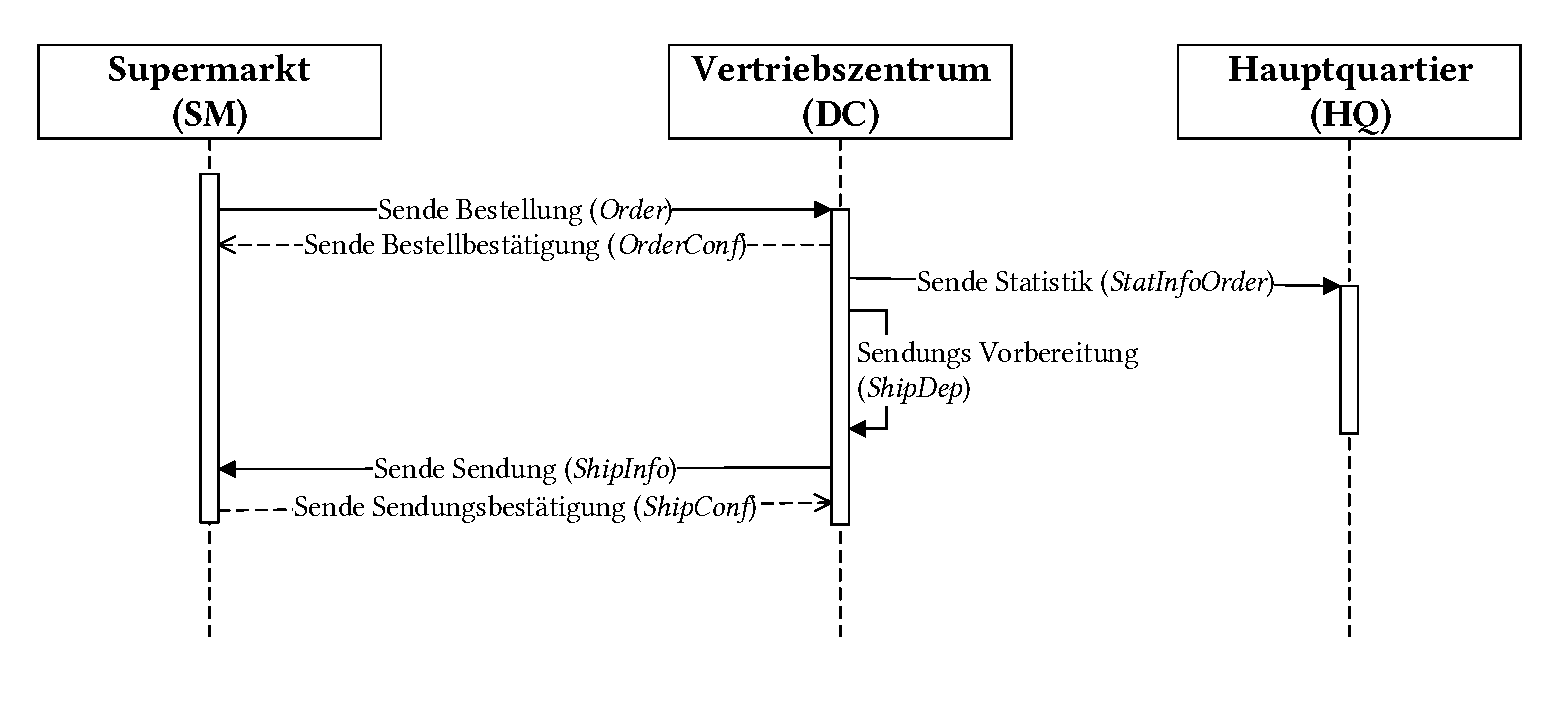
\includegraphics[width=1\textwidth]{images/evaluation/specjms/evaluationInteraktion1seq.pdf}
  \caption{Sequenzdiagramm von Interaktion 1 des SPECjms2007.}
  \label{img:specjmsInteraction1seq}
\end{figure}

\subsubsection{Interaktion 3}
\label{sec:interaction3desc}
Diese Interaktion übt Publisher/Subscriber Kommunikation zwischen dem HQ und seinen SMs aus. Dabei werden persistenten Nachrichten versendet. Es handelt sich um eine Eins-Zu-Viele Kommunikation und wird ausgelöst, wenn die Preise der Ware durch die Firmenleitung (HQ) geändert werden. Um dies zu kommunizieren, sendet das HQ Nachrichten an alle SMs. In \autoref{img:specjmsInteraction3seq} ist der Ablauf der Interaktion als Sequenzdiagramm abgebildet. In der Standardkonfiguration kommuniziert ein HQ mit zehn SMs.
\begin{itemize}
    \item Das HQ sendet ein Preisaktualisierung (\texttt{PriceUpdate}).
    \item Betroffene SMs empfangen und ändern die Information in ihrem System.
\end{itemize}


\begin{figure}
\center
  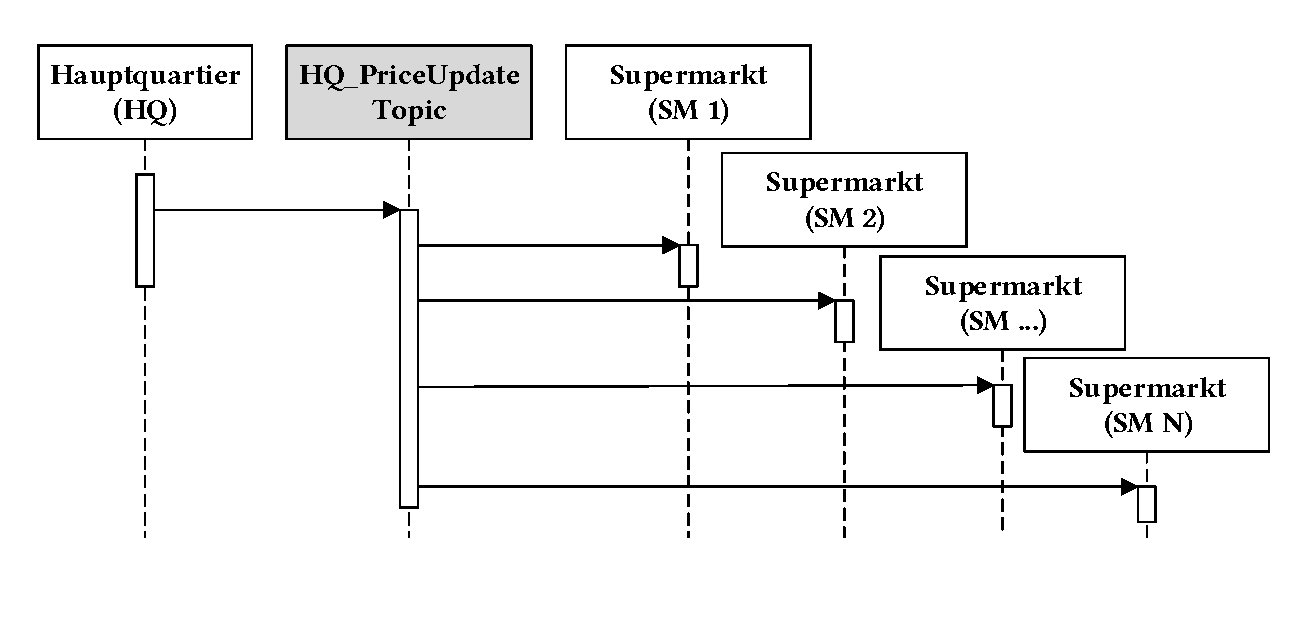
\includegraphics[width=1\textwidth]{images/evaluation/specjms/evaluationInteraktion3seq.pdf}
  \caption{Sequenzdiagramm von Interaktion 3 des SPECjms2007.}
  \label{img:specjmsInteraction3seq}
\end{figure}


\subsection{Konfiguration}
Der SPECjms2007-Benchmark erlaubt verschiedene Konfigurationen durch den Benutzer. Dabei kann die Topologie sowohl horizontal, als auch vertikal skaliert werden. Bei der horizontalen Skalierung, wird die Anzahl der Akteure erhöht, während die Anzahl der gesendeten Nachrichten pro Akteur gleich bleibt. Die vertikale Topologie erhöht die Anzahl der Nachrichten die die Sender senden. Beide Skalierungsarten werden in einer eigenen Konfigurationsdatei mithilfe des Parameters BASE eingestellt.

Außerdem lassen sich für jede Nachricht die Größe und die Verteilung festlegen, mit welcher Wahrscheinlichkeit eine bestimmte Nachrichtengröße auftritt. Die Nachrichtengröße lässt sich mit einer Formel berechnen. Die Formel und ihre Bestandteile wurden in der Arbeit von Sachs et al. \cite{Sachs2013}, mithilfe von Messungen, hergeleitet. Mit folgender Formel lassen sich die Nachrichtengröße berechnen: 
\[m_1 + x * b .\] 
Dabei kann $x$ vom Benutzer des Benchmarks eingestellt werden. Somit kann für jede Nachricht die Wahrscheinlichkeit und ihre Größe festgelegt werden. In \autoref{tab:parameters} sind die für diese Arbeit wichtigen Parameter abgebildet. Die Verteilungen und die dazugehörige Nachrichtengrößen sind in \autoref{tab:msgpropandsize} abgebildet.


\begin{table}
\center
  \begin{tabular}{|c|l|l|l|}
  \hline
    \textbf{Interaktion} & \textbf{Nachricht} & \textit{\(m_1\)} & \textit{b}  \\
    \hline \hline
    \multirow{6}{*}{1} & Order & 0,0565 & 1,4534 \\\cline{2-4}
    & OrderConf & 0,0565 & 1,4534 \\\cline{2-4}
    & ShipDep & 0,0787 & 0,7222 \\\cline{2-4}
    & StatInfoOrder & 0,0153 & 0,1463 \\\cline{2-4}
    & ShipInfo & 0,0787 & 0,8912 \\\cline{2-4}
    & ShipConf & 0,0202 & 0,7140  \\\hline
    \hline
     3 & PriceUpdate & - & 2,310 \\\hline
  \end{tabular}
	\caption{\label{tab:parameters} Parameter zur Berechnung der Nachrichtengröße. Auszug aus Sachs et al. \cite{Sachs2013}.}
\end{table}

\begin{table}
\center
  \begin{tabular}{|c|l|l|l|l|}
  \hline
    \textbf{Interaktion} & \textbf{Nachricht} & \textbf{Größe 1} & \textbf{Größe 2} &\textbf{Größe 3} \\
     & \textit{Wahrscheinlichkeit} & \textit{95\%}  & \textit{4\%} &\textit{1\%}   \\
    \hline \hline
    \multirow{6}{*}{1} & Order & 1,74 & 7,10 & 41,01 \\\cline{2-5}
    & OrderConf & 2,02 & 7,39 & 41,29 \\\cline{2-5}
    & ShipDep & 1,12 & 8,59 & 55,79\\\cline{2-5}
    & StatInfoOrder & 0,22 & 1,67 & 10,83 \\\cline{2-5}
    & ShipInfo & 1,28 & 8,76 & 55,95 \\\cline{2-5}
    & ShipConf & 0,81 & 2,73 & 14,83  \\\hline
    \hline
     3 & PriceUpdate & 0,24 & 0,24 & 0,24 \\\hline
  \end{tabular}
	\caption{\label{tab:msgpropandsize} Nachrichtengröße in KByte. Auszug aus Sachs et al.\cite{Sachs2013}}
\end{table}

\section{Beschreibung der PCM-Modelle}
\label{sec:specjmsmodell}
In der Arbeit von Rathfelder \cite{Rathfelder2013} wurde der SPECjms2007-Benchmark auch als eines von zwei Fallbeispielen verwendet. Dabei ist eine PCM-Modellierung des Systems entstanden. Teile der Modellierung wurden für die Evaluierung dieser Masterarbeit wiederverwendet. Dabei handelt es sich um die Teile, die die Interaktion eins und drei beschreiben. Im Folgenden werden diese PCM-Modell-Teile beschrieben. Außerdem werden Änderungen an den Modellen, sowie ihr Aussehen nach der in \autoref{ch:transformation} beschriebenen Transformation, besprochen. 

\subsection{Repository- und Systemmodell}
Die Akteure, SM, DC, SP und HQ, des Benchmarks sind in der Modellierung jeweils als eine Komponente modelliert. Die einzelnen Nachrichten die durch das System versendet werden, sind jeweils als eigener \emph{EventType} modelliert. Ein \emph{EventType} wird zur Kommunikation zwischen den Komponenten verwendet. Für jede Komponenten wurde eine \emph{SourceRole} und \emph{SinkRole} angegeben, die sich auf den \emph{EventType} bezieht, der gesendet oder empfangen wird. In Abschnitt \ref{img:interaction1system} ist ein Teil des Systemmodells abgebildet, der die Kommunikation der Komponenten für Interaktion 1 beschreibt. Die Interaktion wird durch einen \emph{EntryLevelSystemCall} aus dem Nutzungsmodell gestartet. Im Anschluss werden Nachrichten, wie in Abschnitt \ref{sec:interaction1desc} beschrieben, ausgetauscht. In Abschnitt \ref{img:interaction3system} ist der Teil des Systemmodells abgebildet, der die Interaktion 3 abbildet. Auch hier wird die Interaktion durch einen \emph{EntryLevelSystemCall} aus dem Nutzungsmodell gestartet. Austausch der Nachrichten ist in Abschnitt \ref{sec:interaction3desc} beschrieben. Da es sich bei dieser Interaktion um ein Publish/Subscribe Szenario handelt, wird ein \emph{EventChannel} verwendet um den \emph{EventType} an die Empfänger zu verteilen.

\begin{figure}
\center
  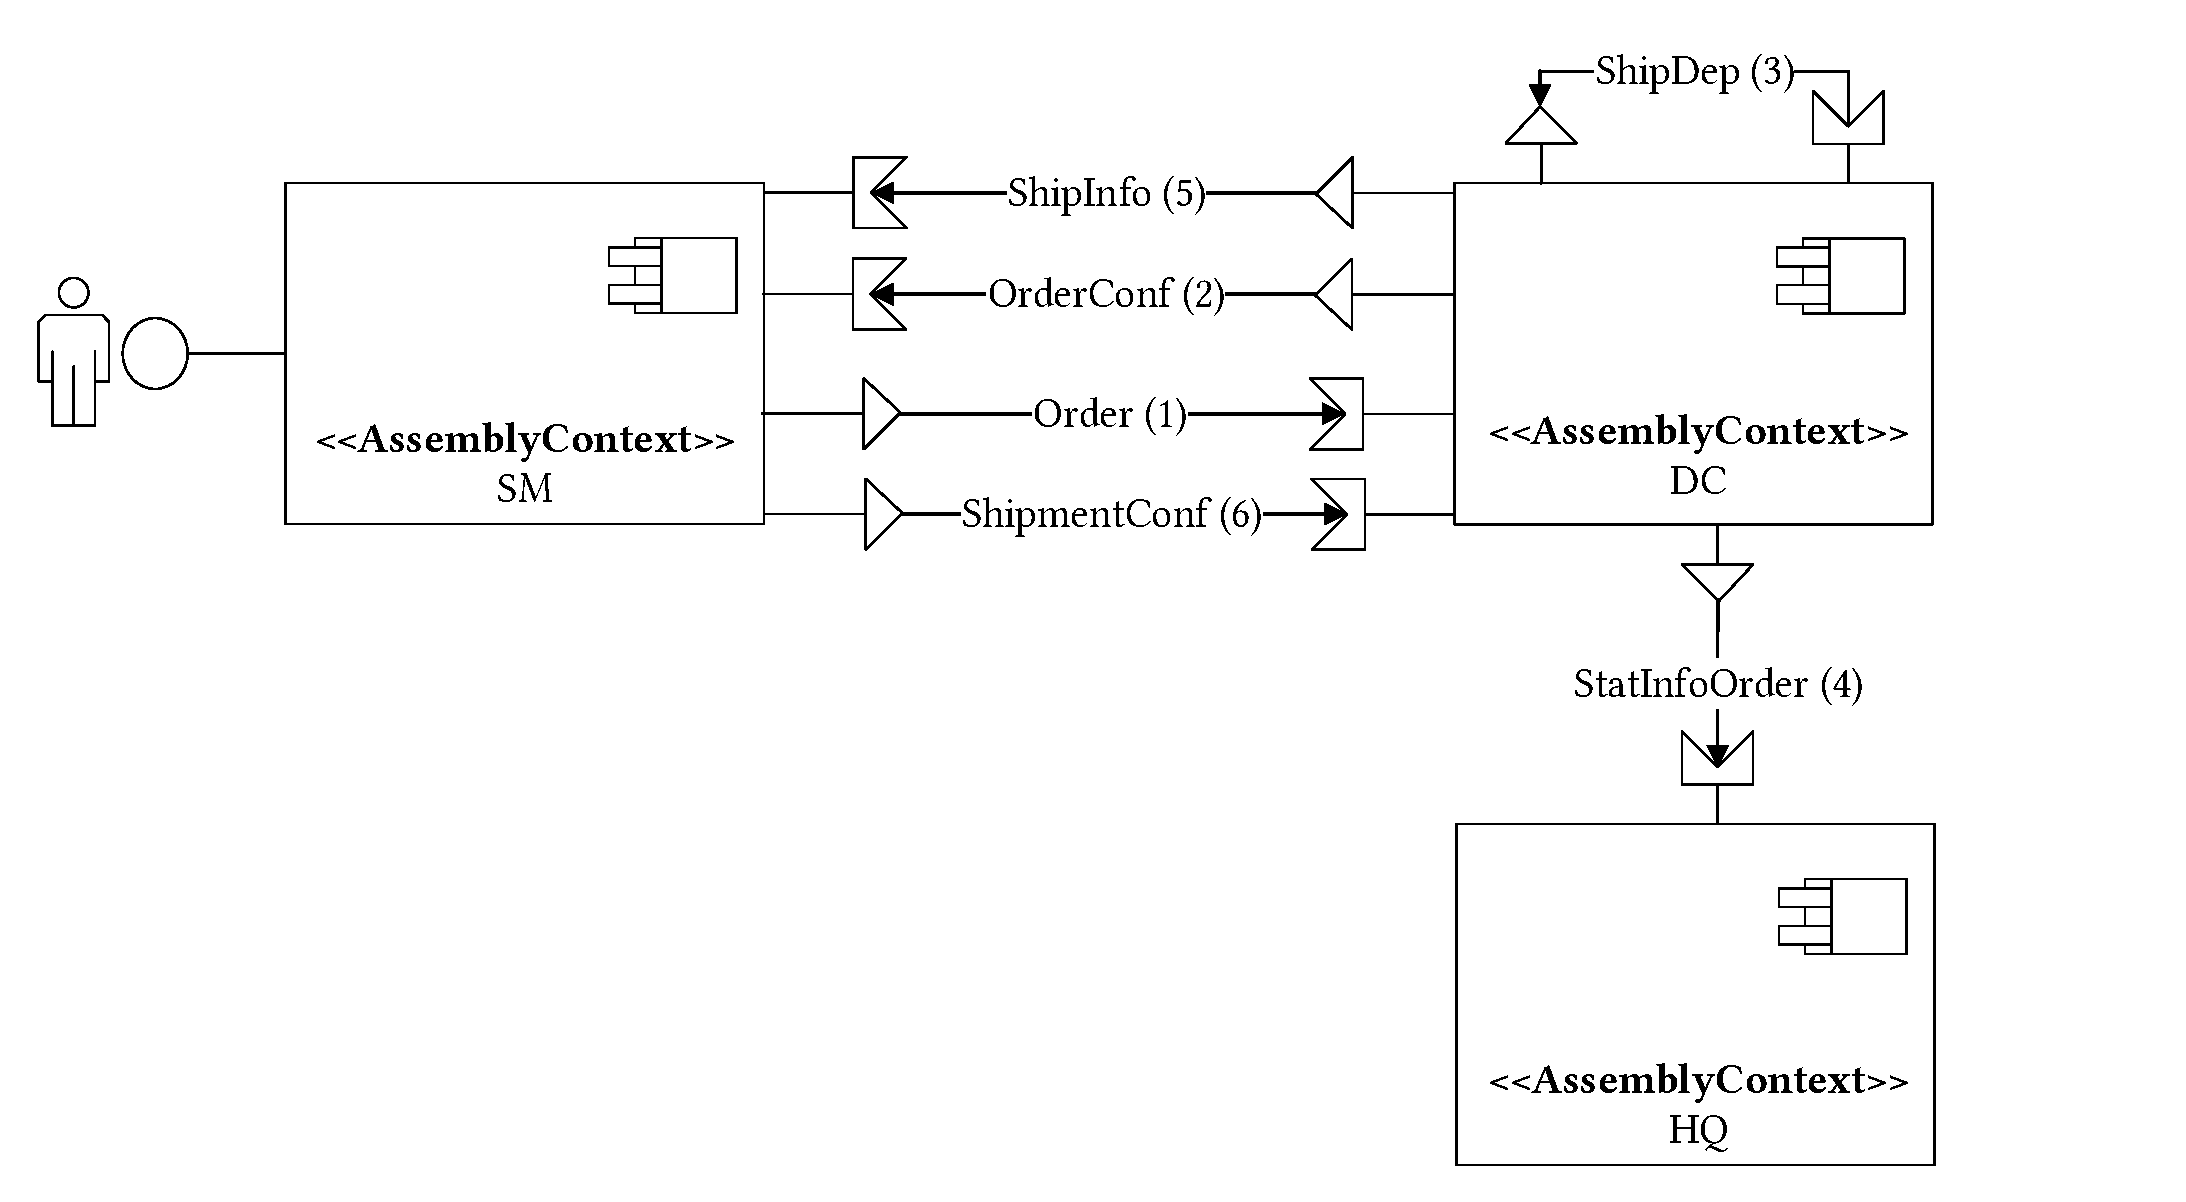
\includegraphics[width=1\textwidth]{images/evaluation/specjms/evaluationInteraktion1events.pdf}
  \caption{Modell der Interaktion 1 des SPECjms2007 mit PCM-Event-Elementen}
  \label{img:interaction1system}
\end{figure}

\begin{figure}
\center
  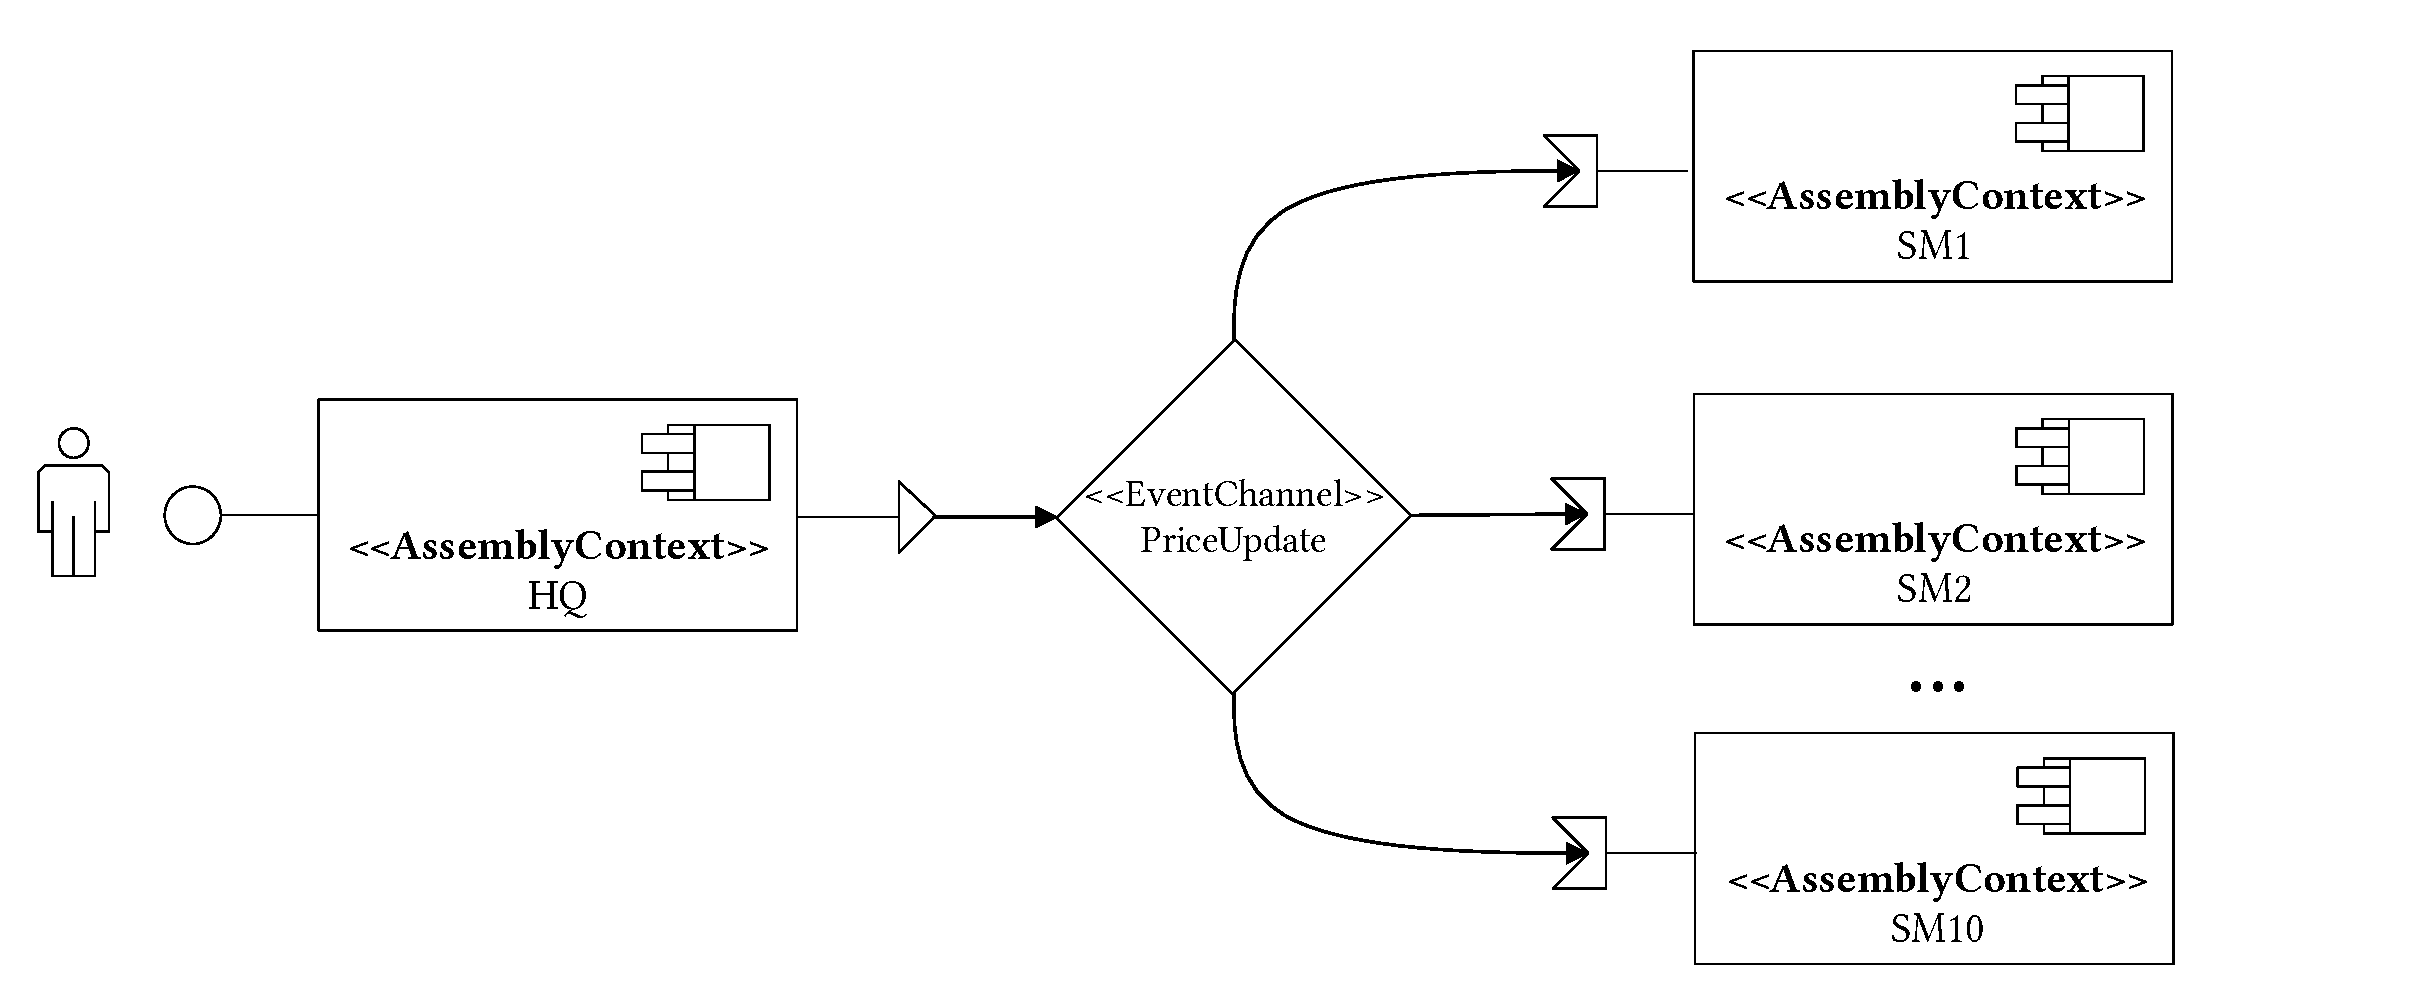
\includegraphics[width=1\textwidth]{images/evaluation/specjms/evaluationInteraktion3events.pdf}
  \caption{Modell der Interaktion 3 des SPECjms2007 mit PCM-Event-Elementen}
  \label{img:interaction3system}
\end{figure}

%\subsection{Ausführungsumgebung und Allokation}

\subsection{Nutzungsmodell}
Das Nutzungsmodell enthält für jede Interaktion ein eigenes \emph{UsageScenario}. Ein \emph{UsageScenario} beinhaltet einen Aufruf, der im Repository-Modell die jeweilige Interaktion startet. Die Verwendung von separaten \emph{UsageScenario}s ermöglicht es, für jede Interaktion eine individuelle Senderate festzulegen. Eine Interaktion kann bei Bedarf auch deaktiviert werden. Die Verteilung der verschiedenen Nachrichtengrößen wird an dieser Stelle als Parameterbelegung eingefügt.

\subsection{MOM}
Zusätzlich enthält die Modellierung des SPECjms2007-Benchmark ein Middleware-Repository. Dieses besteht aus drei Komponenten die die fünf Middleware-Schnittstellen bereitstellen, damit die Middleware in die Systemarchitektur eingewebt wird. Um die Ressourcenanforderung richtig abbilden zu können wurde in der Arbeit von Rathfelder \cite{Rathfelder2013}, für jede Nachricht die Ressourcenanforderung ausgemessen. Anschließend wurde das Middleware-Repository-Modell damit kalibriert. Ein Auszug der Ressourcenanforderungen für die Nachrichten der Interaktionen eins und drei ist in \autoref{tab:specjmsMsgSizeRd} abgebildet. Um die Ressourcenanforderungen im Middleware-Modell zu spezifizieren wurden \emph{BranchAction}s verwendet. Dazu wurde zu jedem Nachrichtentyp eine eigene \emph{BranchAction} angelegt, die die Ressourcenanforderung angibt. 

\begin{table}
\center
  \begin{tabular}{|c|l|l|l|l|}
  \hline
    \textbf{Interaktion} & \textbf{Nachricht} & \textbf{CPU-RD 1} & \textbf{CPU-RD 2} &\textbf{CPU-RD 3} \\
    \hline \hline
    \multirow{6}{*}{1} & Order & 0,973 & 0,987 & 1,846 \\\cline{2-5}
    & OrderConf & 0,390 & 0,365 & 0,663 \\\cline{2-5}
    & ShipDep & 0,539 & 1,148 & 2,494\\\cline{2-5}
    & StatInfoOrder & 0,053 & 0,112 & 0,242 \\\cline{2-5}
    & ShipInfo & 0,616 & 1,170 & 2,501 \\\cline{2-5}
    & ShipConf & 0,390 & 0,365 & 0,663  \\\hline
    \hline
     3 & PriceUpdate & 0,501 & 0,501 & 0,501 \\\hline
  \end{tabular}
	\caption{\label{tab:specjmsMsgSizeRd} Ausgerechnete Ressourcenanforderungen für die Nachrichten. Auszug aus \cite{Rathfelder2013}}
\end{table}



\subsection{Anpassung des Modells}
Während in der Arbeit von Rathfelder jede Nachricht des SPECjms2007 ausgemessen wurde und anschließend über eine Fallunterscheidung in das Middleware-Modell eingesetzt wurde, wurde in dieser Masterarbeit zuerst ein allgemeines System ausgemessen um ein Middleware-Modell zu kalibrieren. Mithilfe dieses Middleware-Modells sollen Vorhersagen über verschiedene Systeme getroffen werden können. Dies ist mit dem Middleware-Repository-Modell aus der Arbeit von Rathfelder nicht möglich, da eine Middleware für ein bestimmtes System ausgemessen wurde. Deshalb wird dieses Middleware-Repository und die darin enthaltene Modellkalibrierung, in der weiteren Evaluierung nicht weiter verwendet und durch den Ansatz aus dieser Masterarbeit ersetzt. 
Die anderen zuvor vorgestellten Modelle werden dagegen wiederverwendet. Außerdem wird eine neue Parameterbelegung für die einzelnen \emph{EmitEventAction}s spezifiziert. Anstelle das die Ressourcenanforderung im Middleware-Modell spezifiziert werden, wird nun die Größe der einzelnen Nachrichten bei der jeweiligen \emph{EmitEventAction}, mithilfe einer Parameterbelegung, spezifiziert. Eine weitere Anpassung ist, dass die Event-Transformation, die das Middleware-Modell in die Systemarchitektur einwebt nicht verwendet wird. Stattdessen werden die Event-Modell-Elemente mithilfe der in \autoref{ch:transformation} vorgestellten Modell-Transformation transformiert. Die Ergebnisse der Transformation werden im Folgenden vorgestellt.



%evtl nachrichtengröße wird in usage modell mit angegeben \\


\subsubsection{Interaktion 1}
In \autoref{img:interaction1systemAfterTransformation} ist der Teil des Systemmodells abgebildet, der die Interaktion 1 darstellt. Zu sehen ist, dass die einzelnen Akteure voneinander entkoppelt wurden und an einen zentralen Exchange angeschlossen wurden. Für jeden Nachrichtentyp (\emph{EventType}) wurde eine Warteschlange angelegt, die ebenfalls an den Exchange angeschlossen wurde. Für die Empfangsaktionen wurde jeweils ein neues \emph{UsageScenario} angelegt, die jeweils die angeforderte Nachricht, sobald sie in der Warteschlange ist, entnehmen. 
\begin{figure}
\center
  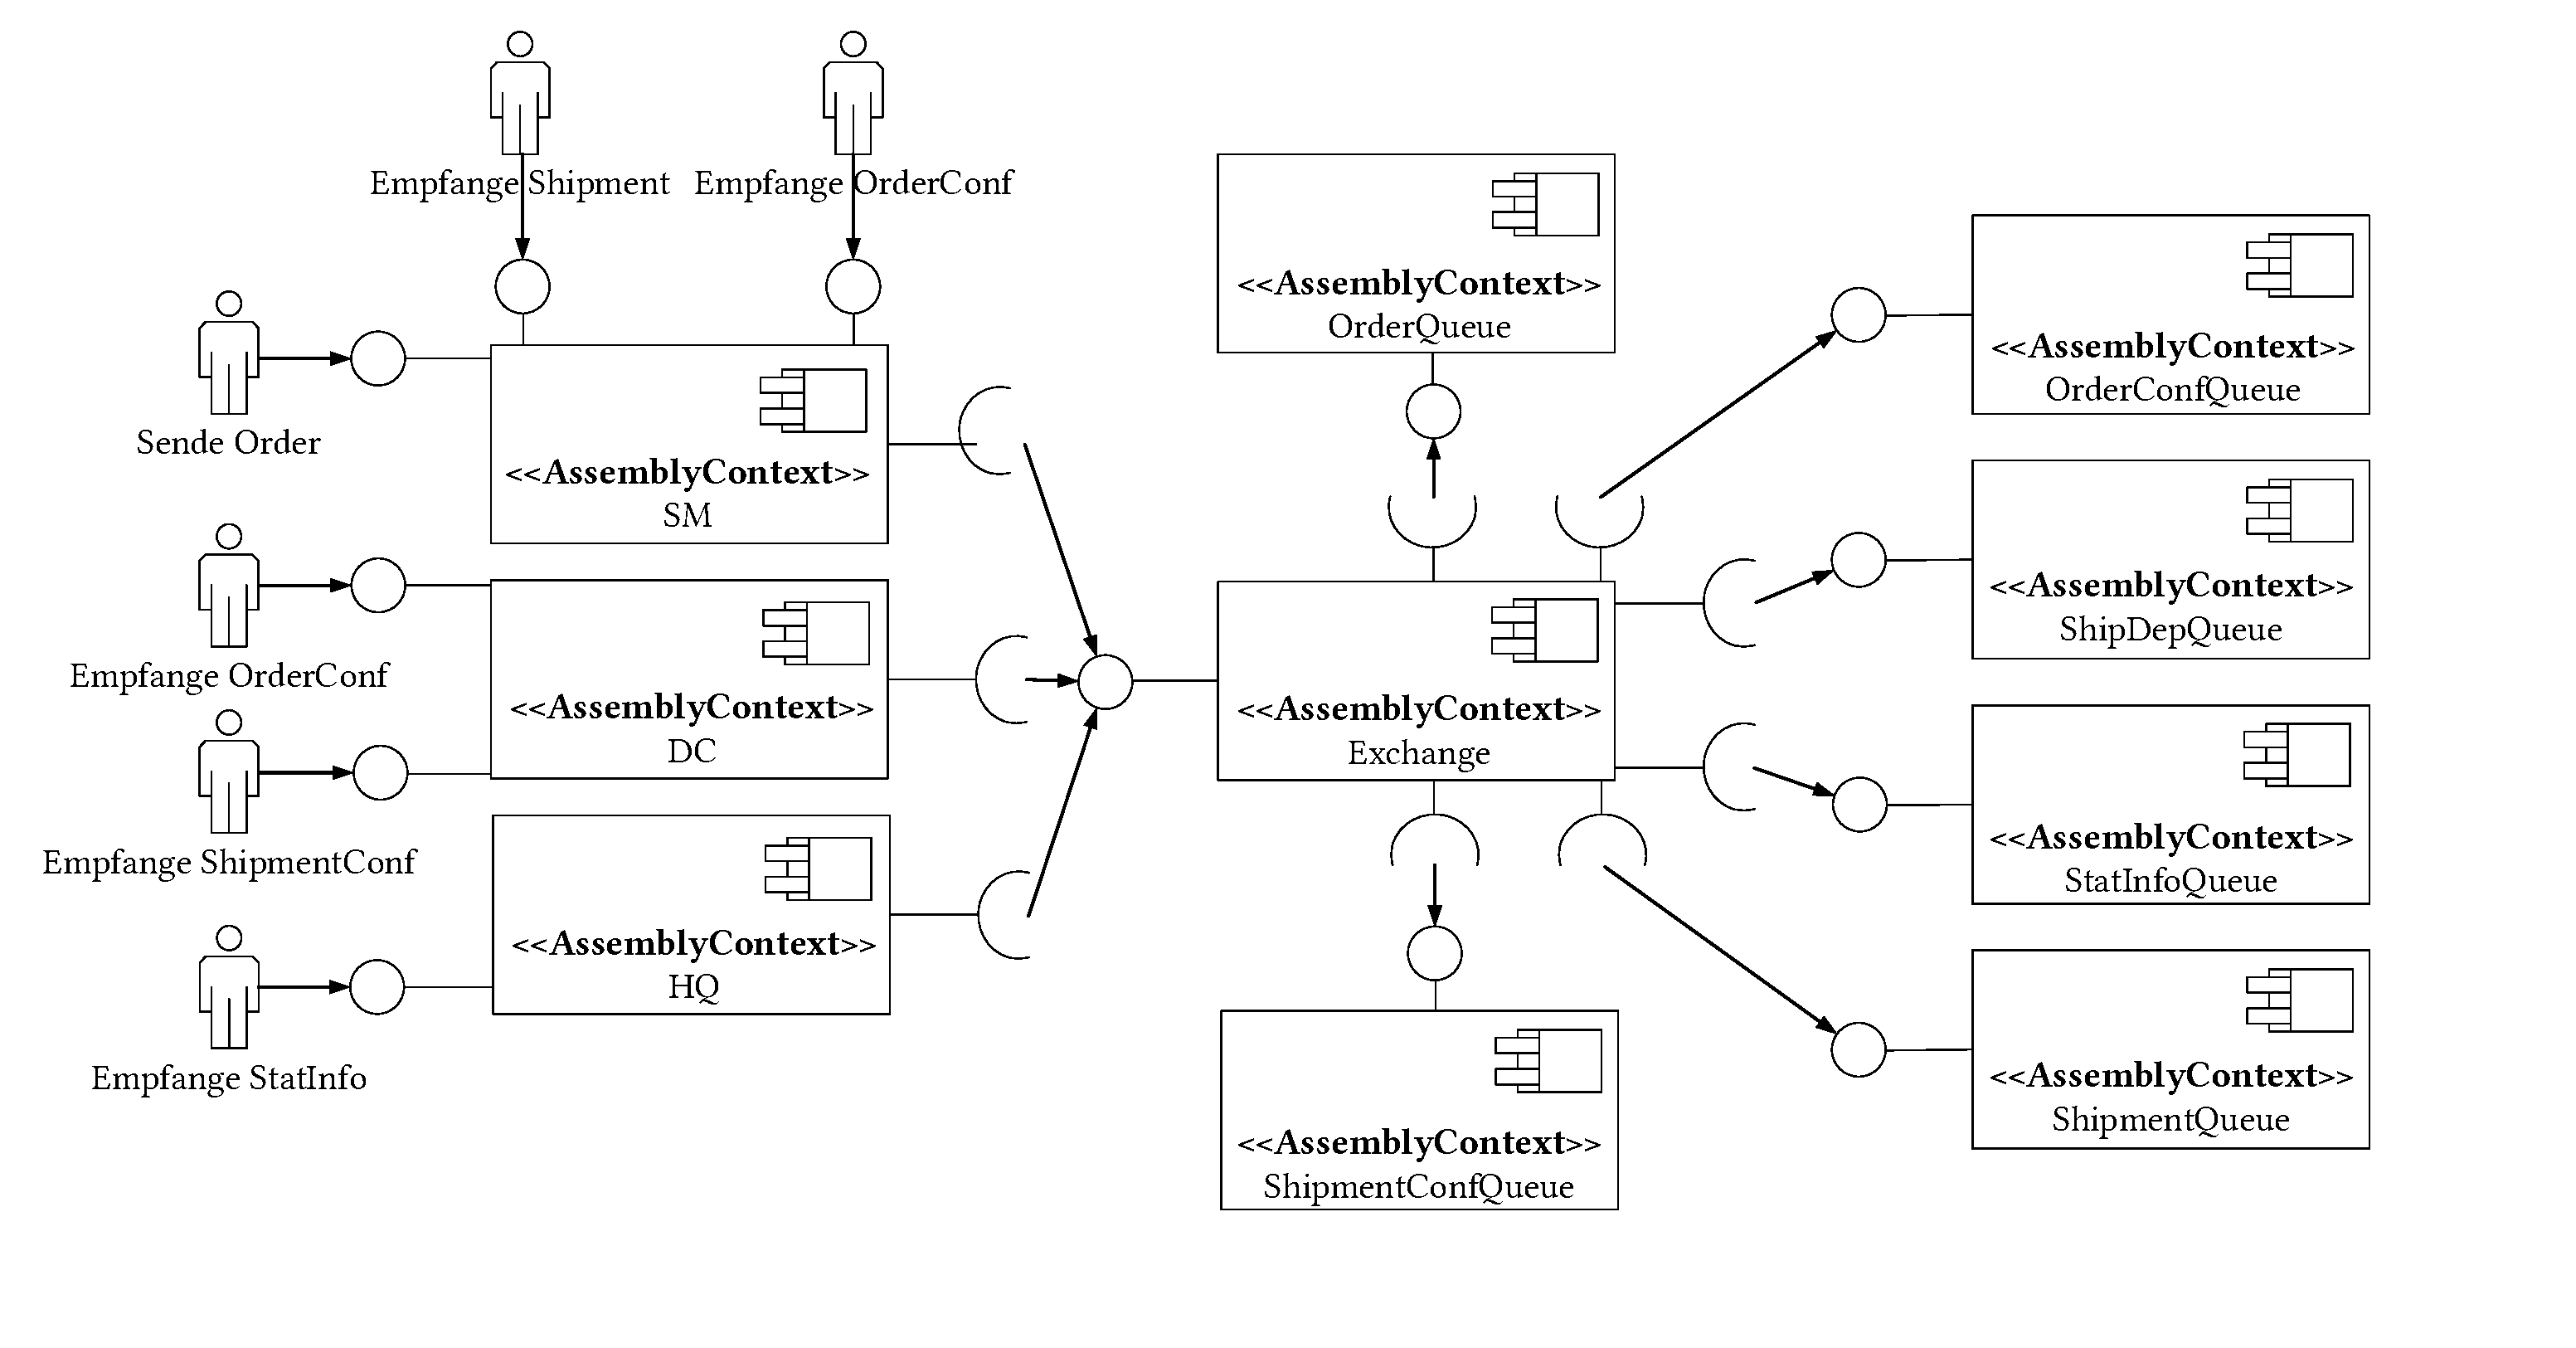
\includegraphics[width=1.4\textwidth,angle=90]{images/evaluation/specjms/evaluationInteraktion1new.pdf}
  \caption{Modell der Interaktion 1 des SPECjms2007 nach der Modelltransformation aus \autoref{ch:transformation}}
  \label{img:interaction1systemAfterTransformation}
\end{figure}
\subsubsection{Interaktion 3}
In \autoref{img:interaction1systemAfterTransformation} ist der Teil des Systemmodells abgebildet, der die Interaktion 3 darstellt. In diesem Fall wurden Empfänger und Sender gemeinsam an den Exchange angeschlossen. Für jeden Empfänger wurde außerdem eine Warteschlange angelegt, die ebenfalls an den Exchange angeschlossen wurde. Die einzelnen Warteschlangen beinhalten jeweils den gleichen Nachrichtentyp, hier \texttt{PriceUpdate}-Nachrichten. Für die Empfangsaktionen wurde jeweils ein neues \emph{UsageScenario} angelegt, die jeweils die angeforderte Nachricht, sobald sie in der Warteschlange ist, entnehmen.
\begin{figure}
\center
  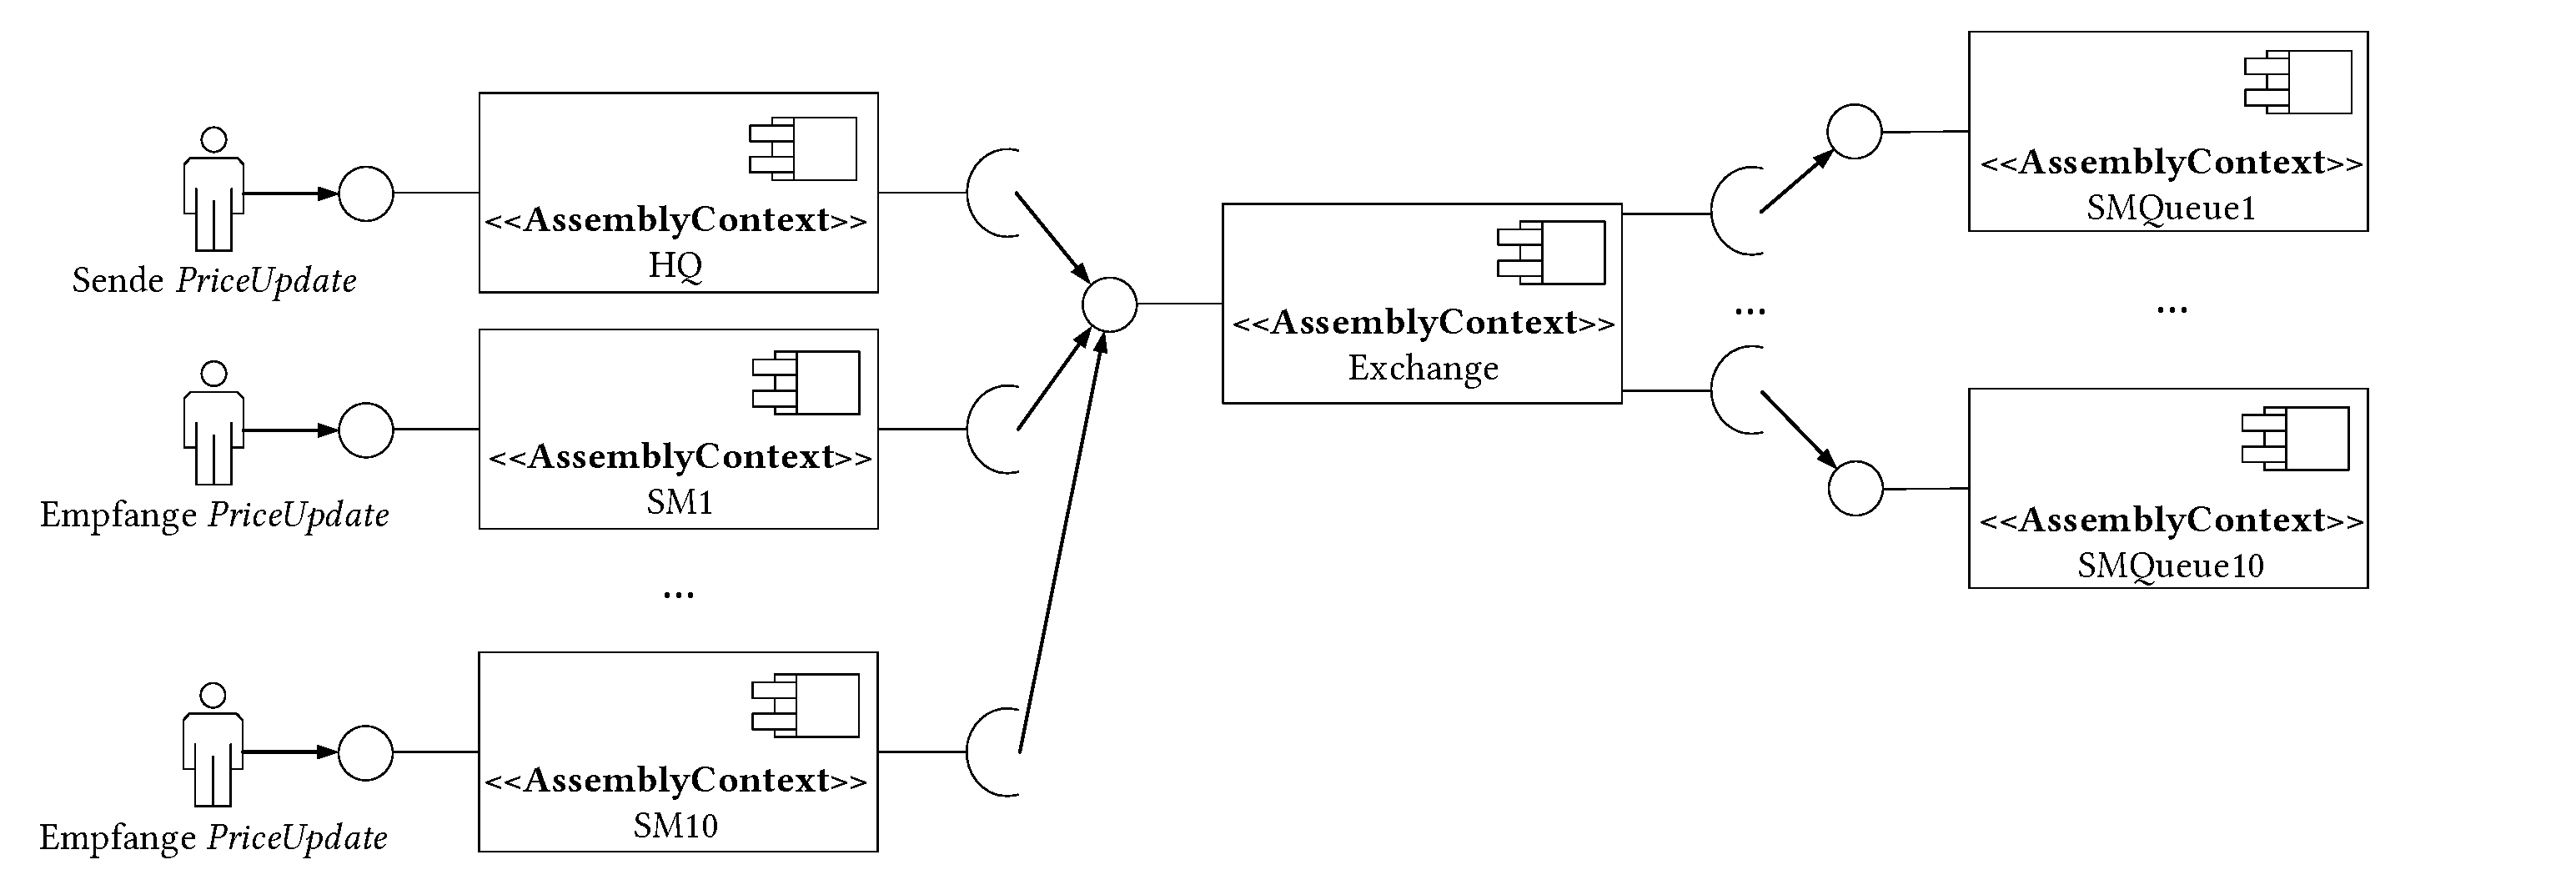
\includegraphics[width=1.4\textwidth,angle=90]{images/evaluation/specjms/evaluationInteraktion3new.pdf}
  \caption{Modell der Interaktion 3 des SPECjms2007 nach der Modelltransformation aus \autoref{ch:transformation}}
  \label{img:interaction3systemAfterTransformation}
\end{figure}


\section{Evaluation der Vorhersagegenauigkeit}
\label{sec:specjmsmodellvorhersage}
Im Folgenden soll die Vorhersagegenauigkeit des Ansatzes dieser Masterarbeit mithilfe des zuvor vorgestellten SPECjms2007-Benchmark und der Modellierung dessen gezeigt werden. Wie bereits erwähnt werden dazu die Interaktionen eins und drei in ihrer, vom Benchmark vorgegebenen, Standardkonfiguration getestet. Als MOM wurde RabbitMQ (RMQ) verwendet. Die einzelnen Messungen starteten mit eine zehn minütigen Aufwärmphase. Im Anschluss wurde eine 30 minütige Messung durchgeführt. Die Dauer wurde aus der Standardkonfiguration des Benchmarks übernommen. Jede Messung wurde zehn mal durchgeführt. Die Experimentumgebung ist, wie schon beim Ausmessen von RMQ, auf einem virtuellen Server ausgeführt worden. Die Spezifikation des Systems ist in \autoref{tab:systespec} abgebildet. Es wurde der Fall betrachtet, dass alle Sender, Empfänger und RMQ sich auf der selben Maschine befinden. Somit wurde der Aufbau wie in \autoref{img:machineoverview}a betrachtet. Für die Vorhersage wurde eine Performance-Analyse mithilfe der Palladio-Bench durchgeführt. Als Analysewerkzeug wurde \emph{SimuCom} verwendet. Im Folgenden werden die Ergebnisse der Messungen und der Vorhersagen aus der Performance-Analyse, für beide Interaktionen und der jeweiligen Konfigurationen, präsentiert. Dazu wird der relative Fehler zwischen dem gemessenen und vorhergesagten Wert, für die Latenz einer Nachricht, berechnet. Die dazu verwendete Formel ist:
\[ Fehler\% = \frac{|Vorhersage - Messung|}{Messung} * 100 \]
Der SPECjms2007-Benchmark liefert für jede Interaktion eine Interaktionszeit, die angibt, wie lange die Interaktion vom Senden der ersten Nachricht, bis zum Empfangen der letzten Nachricht gedauert hat. Außerdem wird für jede Nachricht die gesendet wird, auch die Latenz geliefert. Bei der Präsentation der Ergebnisse werden beide Werte verglichen. Die Performance-Analyse liefert hingegen nur die Latenz der einzelnen Nachrichten. Um eine Annäherung an die Interaktionszeit zu bekommen, werden die jeweils relevanten Ergebnisse aufaddiert.
%CPU Auslastung des Specjms vs. Modellierung\\
%mehrer Messungen für Interaktion => Boxplot, der einen Median zeigt. Mit diesem wird dann das Modell verglichen.
\subsection{Interaktion 1}
Die Messergebnisse für Interaktion 1 des SPECjms2007-Benchmarks und der Performance-Analyse des Modells, sind in \autoref{img:specjminteraction1results} abgebildet. Dabei sind für jede Nachricht die jeweiligen Messergebnisse, der Durchschnittslatenz, eingezeichnet. Außerdem wurde für jede Nachricht der Median eingezeichnet. Die Vorhersage durch die Performance-Analyse wurde auch eingetragen. In \autoref{tab:interaction1error} sind die Fehler für die jeweilige Nachricht eingetragen. Dabei ist zu sehen, dass dieser zwischen 20,76\% und 23,79\% liegt. 

\begin{figure}
\center
  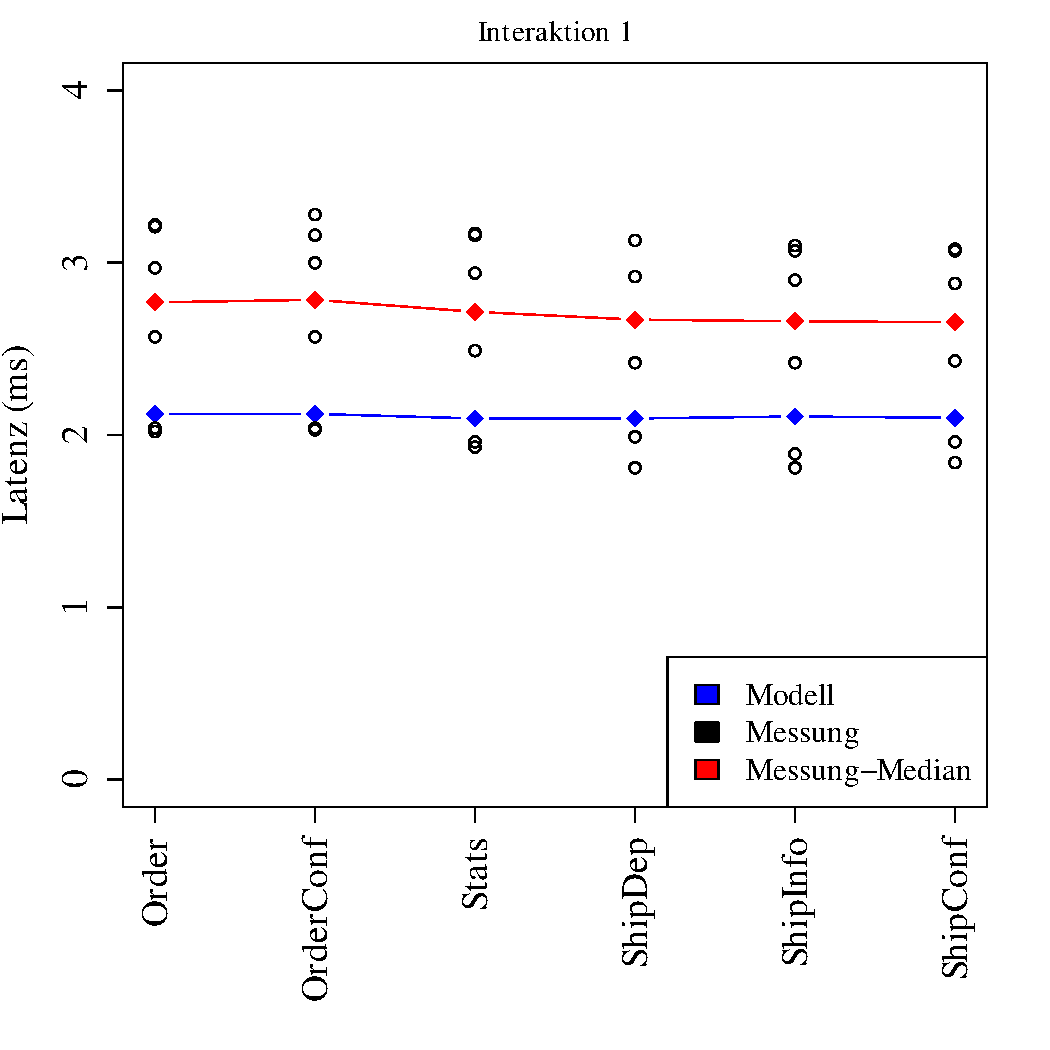
\includegraphics[width=0.6\textwidth]{images/evaluation/specjmsresults/interaktion1.pdf}
  \caption{Latenz der Messung und Vorhersage für die Nachrichten aus Interaktion 1 des SPECjms2007-Benchmark.}
  \label{img:specjminteraction1results}
\end{figure}

In \autoref{img:specjminteraction1interactiontimeresults} ist außerdem ein Boxplot für die gesamte Interaktionszeit abgebildet. Diese setzt sich aus der Latenz der einzelnen Nachrichten wie folgt zusammen: \[\mathit{Order} + max(\mathit{OrderConf}, \mathit{ShipDep}, \mathit{StatInfoOrder}) + \mathit{ShipInfo} + \mathit{ShipConf}\] 
Die Vorhersage der Interaktionszeit aus der Performance-Analyse ist 8,43 ms. Der Fehler zwischen dem Median der gemessenen Interaktionszeit und der Vorhersage beträgt 6,37\%.
%noch mit groesseren Nachrichten \\

\begin{figure}
\center
  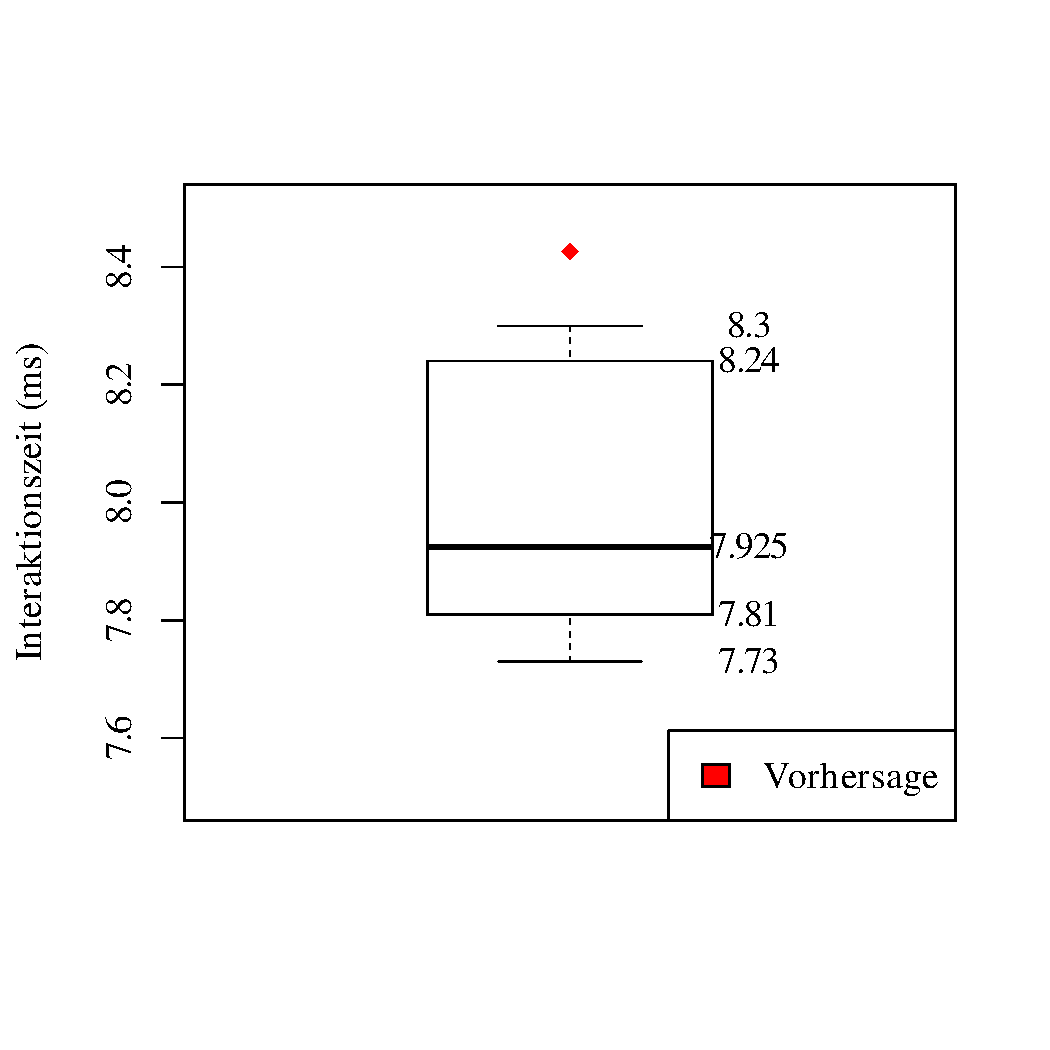
\includegraphics[width=0.6\textwidth]{images/evaluation/specjmsresults/interaktion1InteractionTime.pdf}
  \caption{Boxplot von zehn verschiedenen Messungen von Interaktion 1 des SPECjms2007-Benchmark.}
  \label{img:specjminteraction1interactiontimeresults}
\end{figure}

%\subsubsection{Msg Rate 1}
%Für diesen Vergleich wurde die Senderate der Bestellungen auf eine Bestellung die Sekunde limitiert. Im Anschluss wurde die Interaktion gestartet und nach 10 Minuten beendet. Diese Messung wurde 10 mal durchgeführt. Die durchschnittlichen Interaktionszeiten sind in \autoref{img:specjmsMsgRate1Impl} als Boxplot dargestellt. TODO Boxplot beschreiben. Die Simulation der Modellierung liefert eine Interaktionszeit von 9500 Mikrosekunden (Mit Bild?). Die Fehler sind in \autoref{tab:interaction1msgrate1error} abgebildet. Somit liegt der Fehler fuer diesen Vergleich zwischen 24.66\% und 31.21\%. 

\begin{table}
  \begin{tabular}{|l|c|c|c|c|c|c|}
  \hline
    Nachricht & Order & OrderConf & ShipDep & StatInfo & ShipInfo & ShipConf \\
    \hline
    Messung (ms) & 2,77 & 2,785 & 2,67 & 2,715 & 2,66 & 2,655 \\\hline
    Vorhersage (ms) & 2,12 & 2,12 & 2,1 & 2,1 & 2,11 & 2,1 \\\hline
    Fehler (\%)& 23,36 & 23,79 & 21,5 & 22,8 & 20,76 & 20,91 \\\hline
  \end{tabular}
	\caption{\label{tab:interaction1error} Übersicht der Fehler für Interaktion 1 des SPECjms2007-Benchmark.}
\end{table}

\subsection{Interaktion 3}
In \autoref{img:specjminteraction3results10sm} ist ein Boxplot für die Messungen der Interaktion 3 des SPECjms2007-Benchmark eingezeichnet. Der Median der Latenz, der \texttt{PriceUpdate}-Nachricht, beträgt 4,3 ms. Die Performance-Analyse liefert eine Latenz von 2,1 ms. Der Fehler liegt somit bei 51,16\% und ist somit höher als 40\%, was der in der Literatur akzeptierte Wert ist.

\begin{figure}
\center
  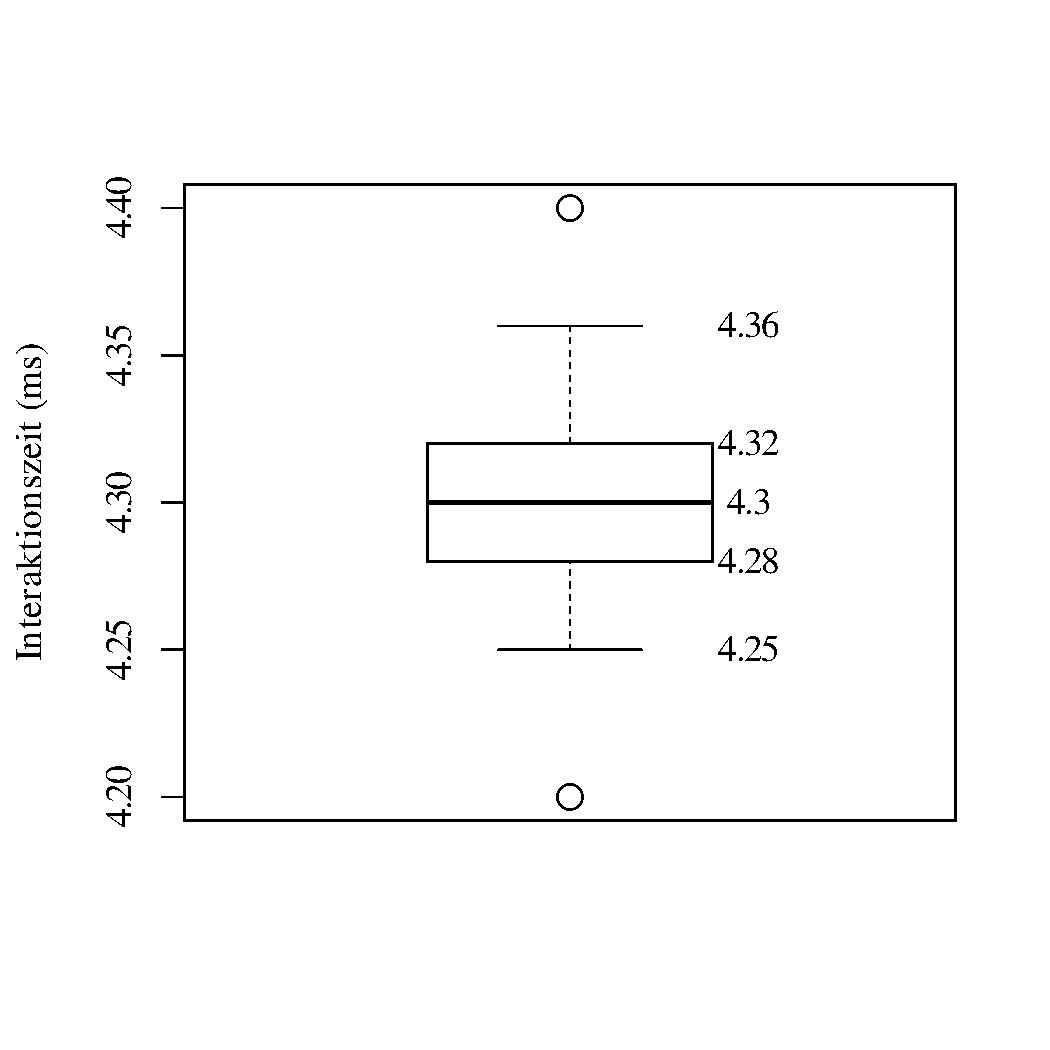
\includegraphics[width=0.6\textwidth]{images/evaluation/specjmsresults/interaktion3-10SM.pdf}
  \caption{Boxplot von zehn verschiedenen Messungen von Interaktion 3 mit zehn Empfängern.}
  \label{img:specjminteraction3results10sm}
\end{figure}

In \autoref{img:specjminteraction3results1sm} wurde der Benchmark nochmal ausgeführt, jedoch mit einem SM, anstatt zehn SMs. Der Median der Latenz beträgt in diesem Fall 2,84 ms. Die Performance-Analyse liefert wieder eine Latenz von 2,1 ms. Der Fehler liegt nun bei 26,06\%. Dies liegt wahrscheinlich daran, dass beim Senden einer Publish/Subscribe-Nachricht eine nicht beachtete Ressourcenanforderung im Exchange stattfindet.
\begin{figure}
\center
  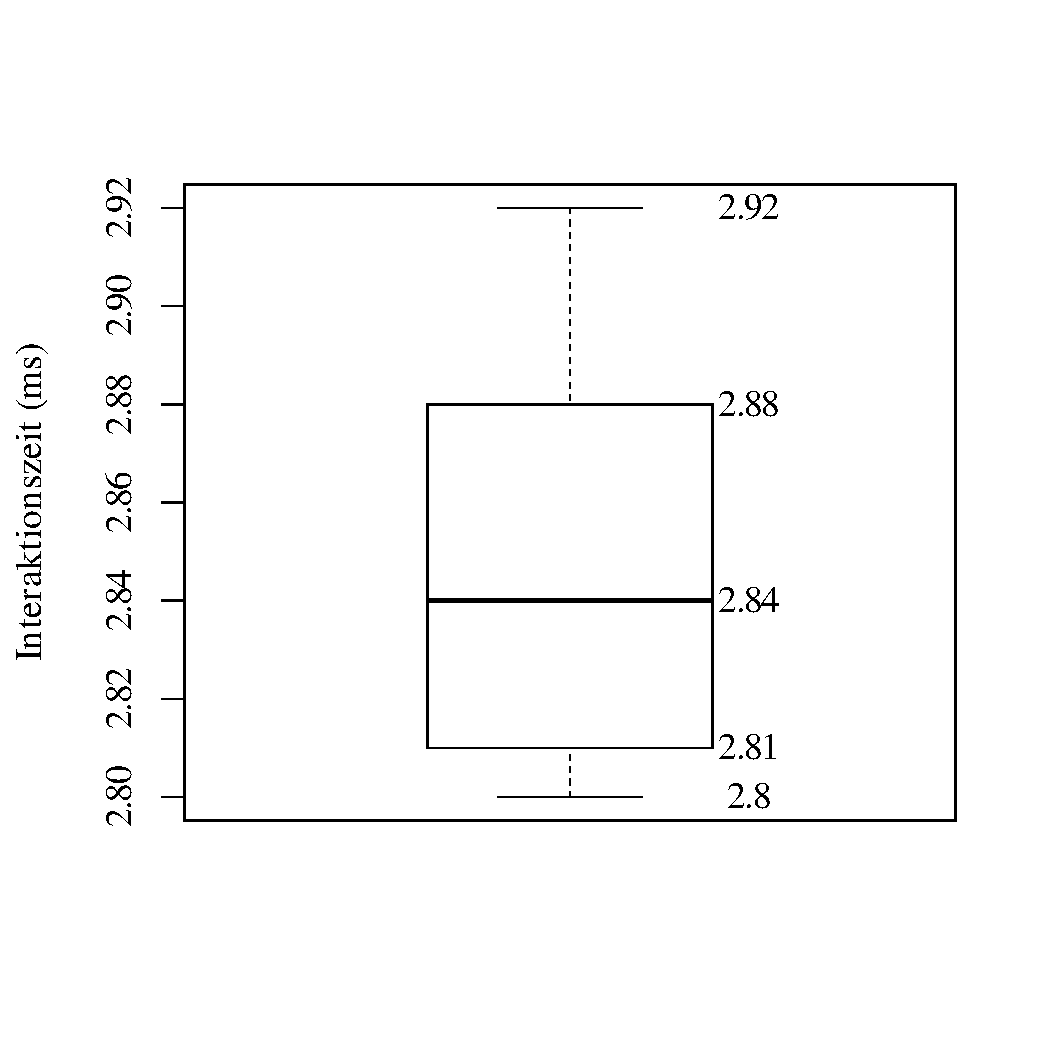
\includegraphics[width=0.6\textwidth]{images/evaluation/specjmsresults/interaktion3-1SM.pdf}
  \caption{Boxplot von zehn verschiedenen Messungen von Interaktion 3 mit einem Empfänger.}
  \label{img:specjminteraction3results1sm}
\end{figure}


\section{Zusammenfassung der Evaluation}
\label{sec:evaluationzusammenfassung}
In diesem Kapitel wurde der Ansatz dieser Masterarbeit mithilfe des SPECjms2007-Benchmark evaluiert. In \autoref{tab:gqm} wurden dazu die Ziele der Evaluierung mithilfe des GQM-Plans formuliert. Im Folgenden wird darauf eingegangen, ob und wie diese Ziele erreicht werden konnten. \par
In \autoref{sec:specjmsmodell} wurden die PCM-Modelle, die den Benchmark modellieren, vorgestellt. Im Anschluss wurden sie mithilfe der Modeltransformation aus \autoref{ch:transformation} transformiert. Dabei konnte gezeigt werden, dass die in \autoref{ch:modellierung} vorgestellte Art eine MOM zu modellieren anwendbar ist. Somit konnte das erste Ziel dieser Arbeit erfüllt werden. 
In \autoref{sec:specjmsmodellvorhersage} wurde die Vorhersagegenauigkeit der Modellierung und ihrer Kalibrierung geprüft. Diese hat gezeigt, dass dies bei einer Punkt-Zu-Punkt-Kommunikation möglich ist, da der Fehler der einzelnen Nachrichten unter 24\% und für die Gesamte Interaktion unter 7\% liegt. Die Vorhersagegenauigkeit für Publish/Subscribe-Kommunikation konnte, mit der aktuellen Kalibrierung, nicht gezeigt werden. Der Fehler beträgt über 40\% und ist somit nicht mehr akzeptiert. Dies zeigt, dass die aktuelle Kalibrierung Publish/Subscribe-Kommunikation nicht unterstützt. Somit konnte das zweite Ziel nur zur Hälfte erreicht werden. \par
In der Arbeit von Rathfelder \cite{Rathfelder2013} liegt der Fehler, der einzelnen Interaktionen, zwischen 20\% und 25\%. Mit dem Ansatz aus dieser Masterarbeit konnte, zumindest für Interaktion 1, eine ähnliche Vorhersagegenauigkeit erzielt werden. Dabei konnte dies erreicht werden ohne die Ressourcenanforderung jeder einzelnen Nachricht auszumessen. 

%Modellierungsaufwand \\

%Modellierung eroeffnet neue moeglichkeiten\\

%\section{TIME}
%Ein weiteres System, das die Anforderungen aus \autoref{sec:systemanforderungen} erfüllt, ist das Transport Information Monitoring Environment (TIME) System \cite{time}. Dabei handelt es sich um ein System der Universität Cambridge. TIME soll ein reales Verkehrsüberwachungssystem darstellen. Es besteht aus mehreren verteilten Komponenten, die verschiedene Arten von Ereignissen senden bzw. empfangen. Die standardmäßige Middleware hat eine Peer-To-Peer Architektur, Punkt-zu-Punkt Kommunikation und unterstützt asynchronen Nachrichtenaustausch. Das System überwacht Autos mithilfe von Kennzeichenerkennung und soll den Verkehrsfluss optimieren. Diese Anwendung ist interessant, weil sie Daten von verschiedenen verteilten Sensoren und Systemen sammelt und integriert. Darüber hinaus enthält es Komponenten mit hohem und unterschiedlichem Ressourcenbedarf, wie z.B. der Kennzeichenerkennungsalgorithmus. Die Systemarchitektur ist sehr anpassungsfähig, wenn es darum geht, neue Komponenten hinzuzufügen oder die Verbindungen zwischen Komponenten oder deren Standort zu ändern. Was dazu führt, dass das hinzufügen und austauschen von verschiedenen MOMs möglich ist. Für die Masterarbeit liegt sowohl die Implementierung, als auch eine PCM-Modellierung des TIME Systems aus einer früheren Arbeit von Christoph Rathfelder \cite{Rathfelder2013} vor. Das TIME System soll für diese Masterarbeit als Evaluierungssystem dienen. Die Modellierung/Implementierung soll zunächst als Referenz für die Performanzanalyse dienen und im nächsten Schritt um verschiedene MOMs erweitert werden.